\chapter{Overview}
\label{chap:overview}

In this section, I provide an overview of some of the essential concepts used in this project, illustrated through the following thought experiment:

Carol, Dave, and Trent are playing a game. In each iteration of the game, Trent will present Carol with some raw data in some format (for example, results of coin flips, or randomly chosen letters) and Carol will try to communicate the data to Dave (who is in the next room) as briefly as possible. Carol and Dave are communicating through a channel that allows only 0s and 1s to be sent. Carol and Dave each know the format of the data and are allowed to coordinate on a strategy for communication before the game starts. In fact, Carol and Dave are so good at this coordination that we may assume that everything Carol knows before the game starts, Dave also knows.

For an example, let us say that the data Trent is presenting to Carol is the result of a sequence of fair coin flips in the format "heads, tails, tails, ..." Because they each know the format, a simple strategy would be to use a \textbf{code} where heads are denoted by 0s and tails are denoted by 1s over their communication channel. We refer to the result of each coin flip as a \textbf{symbol}, and in this example we see that the \textbf{code rate} is 1 bit per symbol.

In this example, symbols are \textbf{independent and identically-distributed random variables (i.i.d.)} because each coin flip has the same 50-50 chance of coming up as heads or tails (identical distribution) and because the result of one coin flip doesn't affect any other (independence).

\section{Information and entropy}
\label{sec:information_and_entropy}

Before attempting to compress a work of literature, let us first think about individual letters.

In another instance of the previous game, Trent presents Carol with a sequence of letters, each randomly chosen from a large English text. As before, symbols are independent and identically-distributed, but in this case, the distribution is not uniform, since the letter E occurs much more often than the letter Q.

As well as saying that Q has a low probability, it is sometimes said that Q has high \textbf{surprisal}. Because of this, Carol and Dave would be wise to privilege the letter E with a short representation in their code (say \texttt{00}), because it will occur often, and vice versa. Because this will leave Q with a longer code, we also say that Q has high \textbf{(self-)information}.

In his seminal paper "A Mathematical Theory of Communication", \textcite{shannon1948mathematical} defines the \textbf{information content} of a symbol as length of its binary representation when the symbol code is chosen optimally (estimated as $-\log p(x)$, where $p(x)$ is the probability of that symbol), and defines the \textbf{entropy} of a random variable (such as our symbols) as the average amount of information per symbol, given by

\[H(X) = \mathbb{E}[-\log p(X)] = -\sum_{x \in \mathcal{X}} p(x) \log p(x)\]

for the discrete random variable $X$. In simple terms, the entropy of a variable is the average number of yes/no questions one needs to ask to determine the value of that variable when choosing one's questions optimally. For a fair coin, one needs to ask only one yes/no question to learn the outcome, and so the entropy of that outcome is 1 bit (sometimes called 1 shannon).

For the English language, the entropy of individual letters based on their frequency is known to be approximately 4.14 bits. This value indicates that, if one person were to select a letter at random from an English text and another person were to try to guess it by asking only yes/no questions optimally, they would need to ask 4.14 questions on average.

The importance of this value is related to Shannon's \textbf{source coding theorem}, given in the same paper, which shows that no code can be chosen for which the code rate is less the entropy of the symbols in question.

In our example with randomly-chosen English letters, the calculated entropy of English letters indicates that no code that Carol and Dave can choose can have a lower code rate than 4.14 bits per symbol. But how might they go about constructing a minimal code?

\section{Entropy coding}

An \textbf{entropy coding} is a consistent way of assigning binary sequences to symbols. Entropy codes usually aim at being minimal in the sense that an encoding of a stream of symbols that the code is designed for should have an average code rate that approximates the symbols' entropy.

The codes are generated from an input mapping between the potential values of each symbol and that value's probability. For example, a coding algorithm may take as its input the mapping $\{A \rightarrow 0.8, B \rightarrow 0.15, C \rightarrow 0.05\}$ and output the mapping $\{A \rightarrow \texttt{0}, B \rightarrow \texttt{10}, C \rightarrow \texttt{11}\}$. Two of the most commonly used entropy codings are Huffman coding and arithmetic coding.

\subsection{Huffman Coding}

\begin{wrapfigure}{r}{0.3\textwidth}
    \centering
    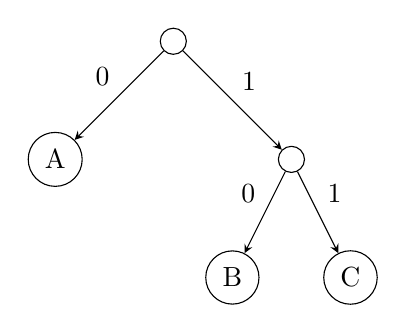
\begin{tikzpicture}
        [->,>=stealth,level/.style={sibling distance = 3cm/#1, level distance = 1.5cm}]
        \node [circle,draw] (root) {} % root node, unlabeled
        child { node [circle,draw] (A) {A} 
            edge from parent node[above left] {0} % Label on the arrow to A
        }
        child { node [circle,draw] (mid) {} % Unlabeled node
            child { node [circle,draw] (B) {B} 
                edge from parent node[above left] {0} % Label on the arrow to B
            }
            child { node [circle,draw] (C) {C} 
                edge from parent node[above right] {1} % Label on the arrow to C
            }
            edge from parent node[above right] {1}
        };
    \end{tikzpicture}
\end{wrapfigure}

Huffman coding works by recursively combining low-probability symbols into a set of symbols that share the same prefix. For example, when given the input $\{A \rightarrow 0.8, B \rightarrow 0.15, C \rightarrow 0.05\}$, Huffman coding combines the symbols B and C into a group that will share the prefix \texttt{1} and which, as a whole, has probability 0.2 .

For this project, I use my own implementation of Huffman coding in the \texttt{Huffman} class available for viewing at \texttt{\href{https://github.com/Guy29/FYP/blob/main/Code/libraries/codes.py}{libraries/codes.py}}.

\todo[inline, color=yellow]{Consider moving the bit about implementation to another section}

\subsection{Arithmetic Coding}

Arithmetic coding is a method where the cumulative probability of symbols is calculated (i.e. $\{\emptyset \rightarrow 0, \{A\} \rightarrow 0.8, \{A,B\} \rightarrow 0.95, \{A,B,C\} \rightarrow 1\}$) and a range within the interval $[0,1)$ is given in a binary format to indicate one of the symbols.

My implementation of arithmetic coding is also available at \texttt{\href{https://github.com/Guy29/FYP/blob/main/Code/libraries/codes.py}{libraries/codes.py}}.

\todo[inline, color=yellow]{Finish writing about this}
\todo[inline, color=yellow]{Consider moving the bit about implementation to another section}

\section{Regularity and the importance of context}
\label{sec:regularity_and_context}

Let's now imagine yet another instance of the game. In this version, the data Trent gives to Carol is a sequence of English letters making up a novel. In this case, our symbols are again letters, and the previously used code for randomly chosen English letters can be used with some success. However, that code is no longer optimal.

This is because the symbols given by Trent are no longer independent or identically distributed, that is, letters cross-correlate. For example, whenever the letter Q appears in the sequence of symbols, there is a high probability that the following symbol will be U, by the structure of English. This \textbf{regularity} can be exploited in Carol and Dave's choice of code, so that whenever the symbol Q is encountered, the symbol U is given a shorter code within that \textbf{context} to reflect its high probability.

In the extreme case where each Q is necessarily followed by a U, Carol and Dave's code may not assign U a code at all, as it can be immediately inferred whenever a Q is encountered. In this case, it can be said that the regularity of QU has been \emph{abstracted out} in the encoded version of the text. The result of this abstraction is a version of the text with less regularity and with higher entropy, that is, a more information-dense representation.

\todo[inline, color=yellow]{Talk a little bit more about why we should expect compressed data to look like noise.}

\section{Prediction and compression}



\todo[inline, color=yellow]{Mention (and maybe include) Shannon's reasoning with the clones.}
\todo[inline, color=yellow]{Somewhere in this report, include and explain Shanon's predictor-interpreter model and visual.}
\todo[inline, color=yellow]{Mention that the value of prediction is that you only have to encode how reality deviates from the prediction}
\todo[inline, color=yellow]{Maybe mention predictive processing, confabulation}

%\section{Practice}
\label{subsec:practice}

\subsection{Tools}

\todo[inline, color=yellow]{For each off these, either relate to the report, move to the section in the report where it's relevant, or delete.}

A variety of compression algorithms are in use today, many of which have been applied to natural language.

\textcite{Mahoney2011} has compiled a document which lists many compression program benchmarks on the \texttt{enwik9} challenge, along with the algorithms and techniques used by each, which is especially relevant to this topic. I touch briefly on each of these below.

\subsubsection{Lempel Ziv and its variations}
These include the original LZ77 \autocite{Ziv1977} and LZ78 \autocite{Ziv1978} algorithms.

\textbf{LZ77}

The first (LZ77) works by replacing repeated substrings inside a larger string with a reference to their first occurrence, indicated by a distance D from the current position at which that occurrence starts and the length L of characters that should be copied from that offset.

For example, the underlined part of the string “CC\textbf{BAABABBBA\underline{B}}\underline{AABABBBAB}BABB” could be represented by (D=9, L=10), indicating that the beginning of the string “CCBAABABBBA” is followed by a 10-character long sequence which is copied from an offset that starts 9 characters back (indicated above in bold).

\textbf{LZ78}

The second algorithm (LZ78) works by incrementally building up a dictionary of previously seen substrings, each composed of a pair of (substring seen even earlier in the text, plus one additional character).

For example, the string “AABABBBABAABABBBABBABB” would be divided into the sections

\begin{center}
\textbf{A}|A\textbf{B}|AB\textbf{B}|\textbf{B}|AB\textbf{A}|ABA\textbf{B}|B\textbf{B}|ABB\textbf{A}|BB
\end{center}

each of which is a previously seen substring plus one additional character (marked in bold). If the sections are numbered 1, 2, 3, etc., the whole string can be abbreviated to

\begin{center}
\textbf{A}|1\textbf{B}|2\textbf{B}|0\textbf{B}|2\textbf{A}|5\textbf{B}|4\textbf{B}|3\textbf{A}|7
\end{center}

In this representation, 1B simply means “the contents of section 1, plus a B”.


\subsubsection{Symbol Ranking}
The SR family of algorithms each keep a ranking of potential symbols, usually as a probability density function. For example, it could estimate a 0.1 probability that a randomly chosen letter is “e” and a 0.01 probability that it is “j”, and consequently assign “e” a shorter code.

This can be done in a rolling fashion where the encoder will update the ranking of the symbols based on how frequent they have been in the text in a sliding window ending at the current symbol, and similarly the decoder will update its own ranking and codebook identically as it is decoding the text. In this case, the codebook keeps changing throughout the text, but both encoder and decoder can construct identical ones based on the text seen so far. 

\subsubsection{Prediction by Partial Matching}
PPM is a SR-based algorithm augmented by conditioning the probabilities of symbols on their “context”, consisting for example of the last n characters read.

If the algorithm has so far read the symbols “aard”, for example, it may estimate a 0.9 probability of the next symbol being “v” and a 0.01 probability of the next symbol being “x”. Based on these estimates, it assigns each of the characters “v” and “x” codes of lengths that correspond to how surprising they would be and will encode the actually observed character using that code.

In decompression, an identical predictor will read the encoded text, create the same codebook, and then use the recorded symbol code to reconstruct the text. \autocite{Fenwick1998}

\subsubsection{Burrows Wheeler Transform}
This algorithm, due to Michael Burrows and David Wheeler \autocite{Burrows1994} acts as an aid to other algorithms which perform better when fed data with runs of repeated characters. The algorithm outputs a reversible permutation of the characters of a string which contains more such runs.

The forward transform works as follows: first, an EOF character is appended to the string, then all circular shifts of the string are calculated and added to an array. This array is then sorted lexicographically, and the concatenation of the last character in each entry of the array is output.

\subsubsection{Dynamic Markov Coding}
Created by Cormack and Horspool \autocite{Cormack1987}. As with SR and PPM, this method of compression uses a predictor which assigns probabilities to potential next tokens, as well as arithmetic coding to assign shorter codes to more likely tokens. Unlike SR and PPM, this method compresses the input one bit at a time, rather than one byte at a time.

\subsubsection{Context Mixing}
Context mixing uses multiple predictors, each using a different context (or features of the text) and each producing its own probability distribution for the next symbol in its input, and combines these probability distributions through one of many possible averaging methods (e.g. linear, logistic) into a unified distribution which is often closer to the true distribution. This results in decoders which are less “surprised” by the next received symbol and which have accordingly assigned it a shorter code. To aid accuracy, CM is implemented in an “adaptive” way, meaning that the weights assigned to each sub-model’s predictions are re-evaluated based on how accurate they’ve been so far. \autocite{Mahoney2005}

\subsubsection{Long Short-Term Memory and Transformers}
LSTMs are a type of recurrent neural network which is fed its previous output as one of its inputs and which maintains an internal state indicating which of its previously seen inputs are relevant to future outputs. Using the attention mechanism, transformers can similarly select relevant parts of an input sequence as context for the part being encoded. Because of their ability to maintain context information, LSTMs and transformers are particularly suited for sequence prediction and so form the basis of another type of predictive coding.
\subsection{Known results}

In 2006, Hutter created a prize to “encourage development of intelligent compressors/programs as a path to AGI” \autocite{Hutter2006}. The challenge is to compress 1GB of text extracted from Wikipedia, chosen because “Wikipedia is an extensive snapshot of Human Knowledge. If you can compress the first 1GB of Wikipedia better than your predecessors, your (de)compressor likely has to be smart(er)” and explaining that “while intelligence is a slippery concept, file sizes are hard numbers.”

The prize is awarded based on improvements in data compression on a specific 1 GB text file, titled \texttt{enwik9}, which is extracted from the English Wikipedia.

The approaches taken by the record holders as well as the performance of their methods gives an indication of the current practical possibilities.

\todo[inline, color=yellow]{Include information about known records and their compression ratios}
\todo[inline, color=orange]{Decide on what to include from the "Practice" file}